\chapter{Three decades of experimental and theoretical work on nanopores}\label{ch:introduction}

\definecolor{shadecolor}{gray}{0.85}
\begin{shaded}
Parts of this chapter were adapted from:\\
\fullcite{Willems-VanMeervelt-2017}
\newpage
\end{shaded}

This chapter serves as a comprehensive introduction to the primary concepts required to understand the
objectives and relevance of the work performed in this thesis. In particular, the reader will be familiarized
with nanopores as single-molecular sensors, and will be given an overview of the relevant experimental and
computational approaches used to investigate their properties. \\
\\
The text and figures of this introductory chapter were entirely written and created by myself.

\newpage



\section{Molecular sensors}
\section{Nanopores as single-molecular sensors}



\section{Nanopore types}

Depending on their constituent material, nanopores are often classified into two distinct groups: the protein-based, \emph{biological} nanopores (BNPs\gls{bnp}) and the semiconductor-based, \emph{solid-state} nanopores (SSNPs\gls{ssnp}).\cite{Dekker-2007} This division runs deeper than the material however, as BNPs are are formed in a bottom-up manner through self-assembly, while SSNPs are fabricated top-down using micromachining techniques. Perhaps the most crucial difference between the two classes is the extent to which they can be modified and manipulated. The proteiaceuous

In recent years, many different types of nanopores have been developed that do not necessarily fall within either category. 





\subsection{Biological nanopores}



Was published \cite{Willems-VanMeervelt-2017}

\subsubsection{\textalpha-HL\textalpha-Hemolysin}

The most widely studied biological nanopore is \textalpha-hemolysin (\gls{ahl}), a homoheptameric porin
secreted by \textit{Staphylococcus aureus}.



\subsubsection{Cytolysin A}

\gls{clya}

\subsubsection{Fragaceatoxin C}

\gls{frac}

\subsubsection{Pleurotolysin AB}

\gls{plyab}

\subsubsection{Other noteworthy biological nanopores}

\subsection{Solid-state nanopores}

\subsection{Hybrid nanopores}



\section{Modelling of biological and solid-state nanopores}
The most commonly used technique to study the complex behavior and properties of biological (i.e. protein) nanopores is molecular dynamics (\gls{md}).

\section{High-throughput nanopore read-out strategies}



% Some dummy code show how to include images.
\begin{figure}
  \centering
  \medskip
  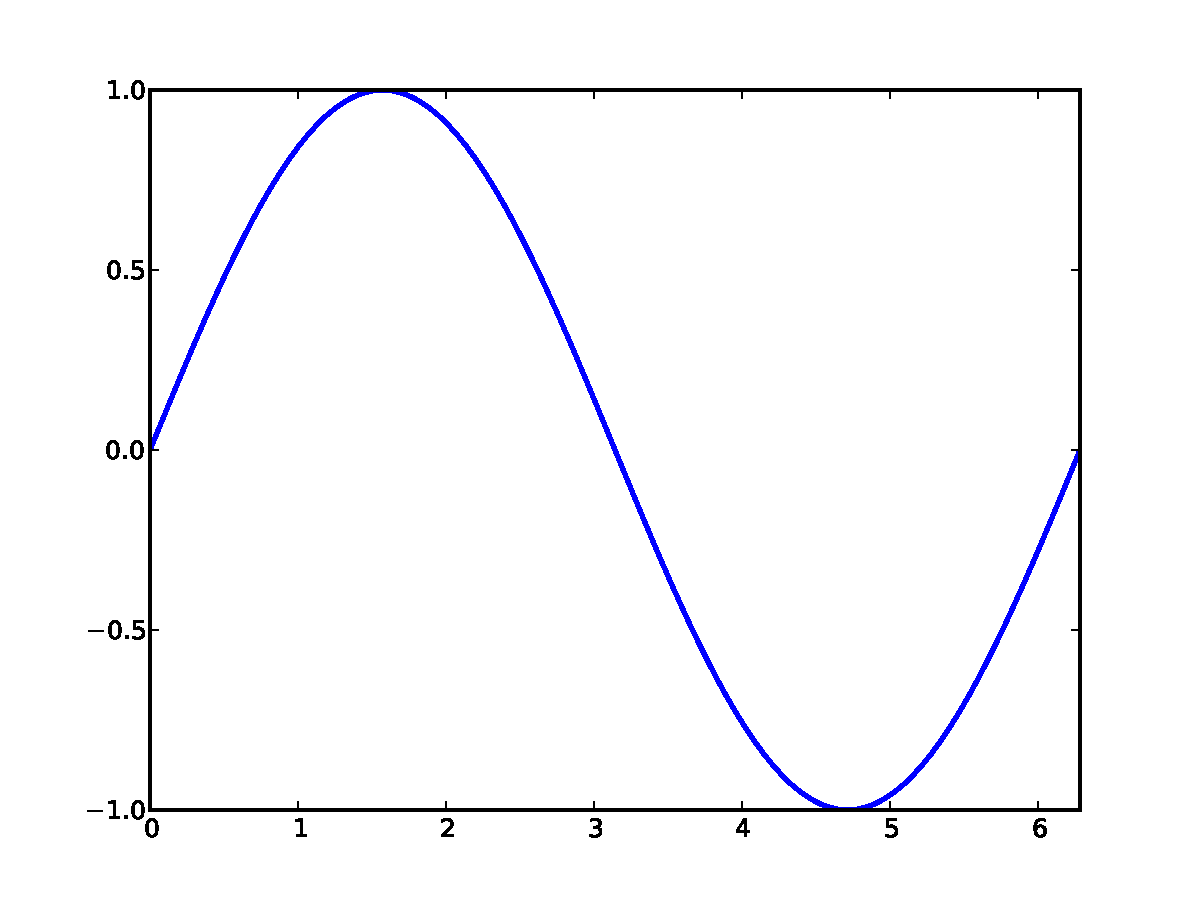
\includegraphics[width=.9\textwidth]{sine}
  \caption{Illustration of how to include a figure. }
  \label{fig:sine}
\end{figure}




%%%%%%%%%%%%%%%%%%%%%%%%%%%%%%%%%%%%%%%%%%%%%%%%%%
% Keep the following \cleardoublepage at the end of this file,
% otherwise \includeonly includes empty pages.
\cleardoublepage

% vim: tw=70 nocindent expandtab foldmethod=marker foldmarker={{{}{,}{}}}
